%//==============================--@--==============================//%
\noindent Curto-circuitos em Sistemas de Energia Elétrica representam uma situação atípica originada por falhas, levando à formação de correntes elevadas. A maioria destes defeitos acontece em linhas aéreas devido à sua grande exposição a fenómenos físicos naturais. Estes podem ser:

\begin{itemize}
    \item \textbf{Trifásicos} quando afetam simultaneamente as três fases do sistema, sendo simétricos no caso de a impedância do defeito ser igual em todas as fases. Se esta impedância for nula, o curto circuito designa-se \textit{franco} (ou \textit{sólido}).

    \item \textbf{Assimétricos} onde podem envolver uma fase e a terra --- curto-circuito fase-terra ou monofásico —, que é o mais habitual, ou duas fases --- curto-circuito fase-fase ---, ou ainda duas fases e a terra --- curto-circuito fase-fase-terra.
\end{itemize}

\noindent Dada a sua perigosidade e potencial de dano a equipamentos, torna-se, por conseguinte, importante desligar no mais curto tempo possível a secção da rede onde se deu o defeito. Esta manobra exige a utilização de interruptores, ditos dijuntores capazes de cortar as correntes de curto-circuito.

%//==============================--@--==============================//%
\subsection{Esquema Monofásico Equivalente}

\noindent Um curto-circuito pode ser modelado pela ligação de uma impedância de baixo (ou nulo) valor no ponto de defeito. Considere-se um defeito trifásico simétrio no barramento \textit{i}, com uma impedância $\mathbf{Z}_{def}$ do qual resultam correntes de curto-circuito iguais em módulo nas três fases e desfasadas de $\pm 120$º. Já que a corrente de curto-circuito é simétrica, podemos usar o esquema monofásico equivalente que se representa na Fig. 34 (b):
\begin{figure}[H]
    \ctikzset{bipoles/length=1.2cm}
    \tikzset{
        line/.style = {line width=1pt, draw=black},
        shin/.style = {line, line width=2pt},
        net node/.style = {circle, draw=black,line width=1.2pt,minimum width=0.8cm, inner sep=0pt, outer 
        sep=0pt},
    }

    \centering
    \begin{subfigure}[b]{0.45\linewidth}
        \centering
        \begin{circuitikz}
        
            \draw[-] (1, 1.5) -- (7.5,1.5) node[yshift=1.7mm,xshift=-63mm] {$a$};
            \draw[-] (1, 1) -- (7.5,1) node[yshift=1.7mm,xshift=-63mm] {$b$};
            \draw[-] (1, 0.5) -- (7.5,0.5) node[yshift=1.7mm,xshift=-63mm] {$c$};
        
            \draw (1.5,0.5) to[generic, l=$\displaystyle \mathbf{Z}_{def}$] (1.5,-1.5);
            \draw (4.25,0.5) to[generic, l=$\displaystyle \mathbf{Z}_{def}$] (4.25,-1.5);
            \draw (7,0.5) to[generic, l=$\displaystyle \mathbf{Z}_{def}$] (7,-1.5);
        
            \draw[-stealth, thick] (1.5, 1.5) -- (1.5,0.1) node[yshift=2mm,xshift=4mm, font=\footnotesize] {$\mathbf{I}_{ai}^{cc}$};
            \draw[-stealth, thick] (4.25, 1) -- (4.25,0.1) node[yshift=2mm,xshift=4mm,font=\footnotesize] {$\mathbf{I}_{bi}^{cc}$};
            \draw[-stealth, thick] (7, 0.5) -- (7,0.1) node[yshift=2mm,xshift=4mm,font=\footnotesize] {$\mathbf{I}_{ci}^{cc}$};
            \draw[dashed] (1,-1.5) -- (7.5,-1.5);
        
        \end{circuitikz}
        \caption{Curto-circuito trifásico simétrico no barramento \textit{i}.}
    \end{subfigure}\hfill
    \begin{subfigure}[b]{0.45\linewidth}
        \begin{circuitikz}
        
            %% Esquema equivalente monofásico
            \path [shin] (1,0.5) -- (7.5,0.5) node[yshift=0mm,xshift=-67mm] {$i$};
            \path [shin] (4.25,1.5) -- (4.25,0.5);
            
            \draw[-] (1.5, 0.5) -- (1.5,-0.5) -- (1,-0.5);
            \draw (7,0.5) to[generic, l=$\displaystyle \mathbf{Z}_{def}$] (7,-1.5);
            \draw[dashed] (1,-1.5) -- (7.5,-1.5);
            
            \draw[-stealth] (4.25, 0.3) -- (4.25,-1.3) node[yshift=8mm,xshift=4mm] {$\mathbf{V}_i^{cc}$};
            \draw[-stealth] (7, 0.2) -- (7,0.1) node[yshift=1mm,xshift=4mm] {$\mathbf{I}_i^{cc}$};
            
            \end{circuitikz}
    \caption{Esquema monofásico equivalente para o defeito.}
    \end{subfigure}

    \caption{Curto-circuito trifásico simétrico}
    \label{fig:transito-dois-barramentos}
\end{figure}

\noindent Usando o \textbf{teorema da sobreposição} é possível considerar o estado da rede após o defeito como a \underline{sobreposição de dois estados}.

\begin{figure}[H]
    \ctikzset{bipoles/length=1.2cm}
    \tikzset{
        line/.style = {line width=1pt, draw=black},
        shin/.style = {line, line width=2pt},
        net node/.style = {circle, draw=black,line width=1.2pt,minimum width=0.8cm, inner sep=0pt, outer 
        sep=0pt},
    }

    \centering
    \begin{subfigure}[b]{0.45\linewidth}
        \centering
        \begin{circuitikz}
            
            %% Esquema equivalente monofásico
            \path [shin] (1,0.5) -- (7.5,0.5) node[yshift=0mm,xshift=-67mm] {$i$};
            \path [shin] (4.25,1.5) -- (4.25,0.5);
        
            \draw[-] (1.5, 0.5) -- (1.5,-1) -- (1,-1);
            \draw[dashed] (7,0.1) to[sinusoidal voltage source, sources/symbol/rotate=auto] (7,-1)  node[yshift=5mm,xshift=7.5mm] {$\mathbf{V}_i^{0}$};
            \node[yshift=0mm,xshift=65mm] (7, 0.5) {$+$};
            \node[yshift=-9mm,xshift=65mm] (7, 0.5) {$-$};
            \draw[dashed] (7,-1) to[generic, l=$\displaystyle \;\;\,\mathbf{Z}_{def}$] (7,-2.5);
            \draw[dashed] (1,-2.5) -- (7.5,-2.5);
        
            \draw[-stealth] (4.25, 0.3) -- (4.25,-2.3) node[yshift=13mm,xshift=4mm] {$\mathbf{V}_i^{0}$};
            \draw[dashed, -stealth] (7, 0.5) -- (7,0.1) node[yshift=1mm,xshift=9mm] {$\mathbf{I} = 0$};
        
        \end{circuitikz}
        \caption{Estado 1.}
    \end{subfigure}\hfill
    \begin{subfigure}[b]{0.45\linewidth}
      \begin{circuitikz}
        
        %% Esquema equivalente monofásico
        \path [shin] (1,0.5) -- (7.5,0.5) node[yshift=0mm,xshift=-67mm] {$i$};
        \path [shin] (4.25,1.5) -- (4.25,0.5);
    
        \draw[-] (1.5, 0.5) -- (1.5,-1) -- (1,-1);
        \draw (7,0.1) to[sinusoidal voltage source, sources/symbol/rotate=auto] (7,-1)  node[yshift=5mm,xshift=7.5mm] {$\mathbf{V}_i^{0}$};
        \node[yshift=0mm,xshift=65mm] (7, 0.5) {$-$};
        \node[yshift=-9mm,xshift=65mm] (7, 0.5) {$+$};
        \draw  (7,-1) to[generic, l=$\displaystyle \;\;\,\mathbf{Z}_{def}$] (7,-2.5);
        \draw[dashed] (1,-2.5) -- (7.5,-2.5);
    
        \draw[-stealth] (4.25, 0.3) -- (4.25,-2.3) node[yshift=13mm,xshift=4mm] {$\mathbf{V}_i^{T}$};
        \draw[-stealth] (7, 0.5) -- (7,0.1) node[yshift=1mm,xshift=7.3mm] {$\mathbf{I}_{ci}^{cc}$};
    
    \end{circuitikz}
    \caption{Estado 2.}
    \end{subfigure}

    \caption{Teorema da sobreposição sob os dois estados do barramento}
    \label{fig:transito-dois-barramentos2}
\end{figure}

\begin{enumerate}
    \item O \textbf{estado 1} corresponde à situação pré-defeito. Uma vez que a f.e.m do gerador fictício é igual à tensão no barramento, a corrente é nula, pelo que pode ser retirado.

    \item O \textbf{estado 2} corresponde à ligação do gerador fictício com polaridade invertida. Os geradores reais são representados unicamente pelas respetivas impedâncias internas.
\end{enumerate}
%//==============================--@--==============================//%
\subsection{Teorema de Thévenin}

O \textbf{estado 2} corresponde à aplicação do teorema de Thévenin, o qual permite estabelecer para uma rede elétrica, vista de qualquer nó $i$, o esquema equivalente representado na Fig. 36, onde $Z_T$ é a impedância equivalente (de Thévenin) da rede vista do nó $i$ quando se anulam as fontes de tensão e/ou de corrente e $V_i^0$ é a tensão pré-defeito.

\vspace{-1em}
\begin{minipage}[b]{.45\linewidth}
\begin{figure}[H]
    \begin{circuitikz}[scale=1]
        \draw (1,0) to[sinusoidal voltage source, sources/symbol/rotate=auto] (7.5,0)  node[yshift=7mm,xshift=-32mm] {$\mathbf{V}_i^{0}$};
        \node[circ] at (2.5, 0) {};
        \node[] at (2.5, 0.2) {$i$};
        \draw  (1,0) to[generic, l=$\displaystyle \mathbf{Z}_{T}$] (1,-4);
        \draw  (7.5,0) to[generic, l=$\displaystyle \mathbf{Z}_{def}$] (7.5,-4);
        \draw[-stealth] (7.5, 0) -- (7.5,-0.8) node[yshift=1mm,xshift=4mm] {$\mathbf{I}_{ci}^{cc}$};
        \draw (1,-4) -- (7.5,-4);
        
        \node[yshift=0mm,xshift=-5mm] at (4.25, 0.5) {$-$};
        \node[yshift=0mm,xshift=5mm] at (4.25, 0.5) {$+$};
    \end{circuitikz}
    \caption{Esquema Equivalente de Thévenin.}
\end{figure}
\end{minipage}\hfill
\begin{minipage}[b]{.45\linewidth}
 \begin{figure}[H]
    Com defeito no nó $i$ com impedância $\mathbf{Z}_{def}$, $\mathbf{I}_{cc}$ é:
    $$
        \mathbf{I}_{cc} = \frac{\mathbf{V}_i^0}{\mathbf{Z}_{def} + \mathbf{Z}_T}
    $$
    Para um sistema trifásico (em unidades do S.I.) será:
    $$
       \mathbf{ I}_{cc} = \frac{\mathbf{V}_i^0}{\sqrt{3}(\mathbf{Z}_{def} + \mathbf{Z}_T)}\;\rightarrow\;
        \boxed{I_{cc} = \frac{\mathbf{V}_i^0}{\sqrt{3}\mathbf{Z}_T}}
    $$
    Sendo $\mathbf{Z}_{def}$ nula (curto-circuito franco):
\end{figure}
\end{minipage}

\vspace{1em}
\noindent Define-se a potência de curto-circuito $S_{cc}$ no nó $i$ por:
$$
    S_i^{cc} = \sqrt{3} V_i^0 I_i^{cc} = \frac{{V_i^0}^2}{Z_T}
$$
Se se tomar para $V_i^0$ a tensão nominal $V_n$:
$$
    S_i^{cc} = \frac{V^2_n}{Z_T}
$$
Em valores p.u.:
$$
    \boxed{S_i^{cc} = I_i^{cc} = \frac{1}{Z_T}}
$$
isto é, \underline{a corrente e a potência de curto-circuito são iguais ao inverso da impedância equivalente da rede} vista do ponto de defeito.
%//==============================--@--==============================//%
\subsection{Curto-Circuito de um Gerador Síncrono}

Considere um gerador síncrono que opera à velocidade nominal, sem carga, excitado por uma corrente constante. Se um curto-circuito trifásico ocorrer no instante $t=0$, a corrente é dada por:
$$
    i_{cc} = \sqrt{2} \frac{E}{X_d'} \cos(\omega t + \alpha_0) - \frac{E}{\sqrt{2}}  \left( \frac{1}{X_d'} + \frac{1}{X_q} \right) \cos \alpha_0 - \frac{E}{\sqrt{2}}  \left( \frac{1}{X_d'} - \frac{1}{X_q} \right) \cos(2\omega t + \alpha_0)
$$
em que as grandezas representam: $X_d'$: reactância transitória ao longo do eixo $d$; $X_q$: reactância síncrona ao longo do eixo $q$; $E$: f.e.m. da máquina; $\omega$: frequência angular nominal; $\alpha_0$: ângulo do rotor no instante do curto-circuito.

\vspace{0.5em}
\noindent Verifica-se portanto que:
\begin{itemize}
    \item A corrente de curto-circuito tem três componentes: uma componente fundamental, uma componente contínua e uma com dupla frequência.
    \item A componente contínua varia com a posição do rotor no momento do defeito.
    \item Desconsiderando as resistências dos enrolamentos, as componentes da corrente de curto-circuito são constantes.
    \item O valor eficaz da componente fundamental é $E/X_d'$. Em regime estacionário, o curto-circuito é maior que a corrente estacionária.
\end{itemize}

\noindent Após a ocorrência de um curto-circuito, o fluxo magnético no gerador não desaparece de imediato, ao contrário do que poderíamos intuitivamente pensar. Uma das principais razões para esta persistência do fluxo magnético é a presença de barras de cobre localizadas na superfície do rotor. Estas barras desempenham um papel crucial na manutenção de um fluxo magnético residual.

\noindent Em situações normais, quando o gerador opera em regime estacionário, o enrolamento no rotor não é percorrido por corrente. No entanto, quando ocorre um desequilíbrio, como no caso de um curto-circuito, a máquina começa a experimentar oscilações que são resultantes de desequilíbrios de potência. Estas oscilações podem ser atribuídas, em parte, à indução de correntes nestes enrolamentos devido às flutuações no fluxo magnético. Estas correntes induzidas atuam como um amortecedor, ajudando a estabilizar a máquina.

Adicionalmente, é imperativo mencionar a reatância subtransitória $X_d^{\prime\prime}$. Durante um curto-circuito, o comportamento do gerador é amplamente influenciado por esta reatância, particularmente nos primeiros ciclos do evento. A reatância $X_d^{\prime\prime}$ reflete a resposta rápida do gerador ao distúrbio, determinada em grande parte pelas correntes no enrolamento amortecedor. Estas correntes, em combinação com a reatância subtransitória, determinam a magnitude inicial e a dinâmica da corrente durante o curto-circuito como apresentado:

\begin{figure}[H]
    \centering
    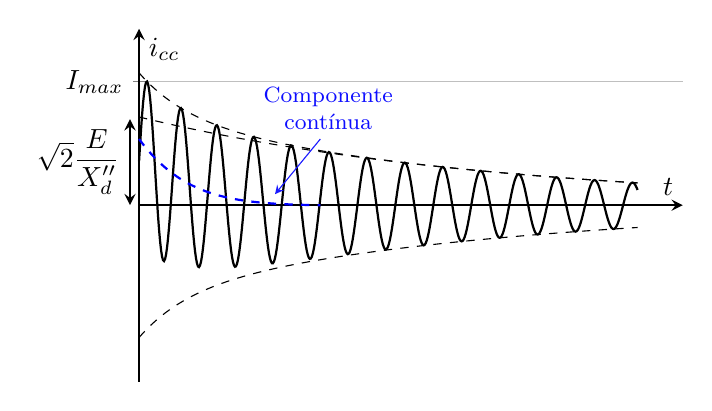
\begin{tikzpicture}
        \begin{axis}[
            axis lines=middle,
            xlabel={$t$},
            ylabel={$i_{cc}$},
            xmin=0, xmax=3, xtick=\empty,
            ymin=-4, ymax=4, ytick={2.8}, yticklabel={$I_{max}$},
            axis line style={thick},
            grid=both, minor tick num=1,
            width=0.7\textwidth,
            height=0.5\textwidth,
            samples=500,
            clip=false,
        ]

        % Parameters (change these to fit your data)
        \def\alpha{0.5}
        \def\omega{30}
        \def\A{1}
        \def\B{1}
        \def\phi{-90}

        % Damped sinusoidal waveform with decaying DC component
        \addplot[black, thick, domain=0:2.75] { exp(-\alpha*x) * 2*\A*cos(deg(\omega*x) + exp(-7.5*\alpha*x) * \phi) + exp(-7.5*\alpha*x) * \B };

        \addplot[dashed, domain=0:2.75] { 2*exp(-\alpha*x) + exp(-7.5*\alpha*x) * \B };
        \addplot[dashed, domain=0:2.75] { 2*exp(-\alpha*x) };
        \addplot[dashed, domain=0:2.75] { -2*exp(-\alpha*x) - exp(-7.5*\alpha*x) * \B };
        \addplot[dashed, blue!, thick, domain=0:1] {ln(x+2) * exp(-8.88*\alpha*x) * \B * 1.5 * 1/ln(2) * (-x*x+1)};
            
        % Vertical arrow denoting the value 1.5, next to the y-axis
        \draw[>=stealth, <->, thick] (-0.05,0) -- (-0.05,1.95) node[midway,left] {$\sqrt{2} \displaystyle\frac{E}{X_d''}$};

        \draw[>=stealth, ->, blue!90] (1,1.5) -- (0.75,0.25);
        \node[blue!95, above, xshift=1mm, align=center, font=\footnotesize] at (1,1.5) {Componente\\contínua};
        
        \end{axis}
    \end{tikzpicture}
\end{figure}

\noindent A corrente que circula no estator durante o curto-circuito também é afetada. De fato, nas primeiras alternâncias após o início do curto-circuito, observa-se um aumento substancial na corrente no estator. Uma das principais contribuições para este aumento é a componente contínua da corrente. A sua presença resulta num acréscimo significativo no valor de pico das primeiras alternâncias da corrente de curto-circuito. Em termos numéricos, este aumento pode chegar a ser até $1.8\sqrt{2} = 2.55$ vezes o valor eficaz da componente alternada. É crucial entender a interação entre esta componente contínua e a corrente alternada, uma vez que determina a resposta dinâmica da máquina em situações de falha e influencia as medidas de proteção a serem adotadas. 

O efeito desmagnetizante desta corrente, que tende a enfraquecer o fluxo, é compensado por um aumento da corrente do enrolamento de excitação, que tem um efeito magnetizante. Dado que este enrolamento tem uma resistência não nula, esta corrente vai diminuindo com uma constante de tempo \(T_d'\) (aproximadamente \(T_d' \approx T_{d0}' \cdot X_d'/X_d''\)), onde \(T_{d0}'\) é a constante de tempo do enrolamento de excitação (da ordem de 5-10 s). Isto origina um enfraquecimento do fluxo no entreferro e, portanto, da tensão do gerador. A corrente no estator vai, consequentemente, diminuindo também até atingir o seu valor em regime estacionário com uma constante de tempo \(T_d'\) (cerca de 1-2 s).

\begin{figure}[H]
    \begin{subfigure}[b]{.475\linewidth}
        \centering
        \begin{tikzpicture}
            \begin{axis}[
                axis lines=middle,
                xlabel={$t$},
                ylabel={$\phi$},
                xmin=0, xmax=5, xtick=\empty,
                ymin=0, ymax=5, ytick=\empty,
                axis line style={thick},
                grid=both, minor tick num=1,
                width=\textwidth,
                samples=500,
            ]

            \addplot[black, thick] {1.75*exp(-0.5*x)+1.05};
            
            \end{axis}
        \end{tikzpicture}
    \end{subfigure}\hfill
    \begin{subfigure}[b]{.475\linewidth}
        \centering
        \begin{tikzpicture}
            \begin{axis}[
                axis lines=middle,
                xlabel={$t$},
                ylabel={$i_r$},
                xmin=0, xmax=5, xtick=\empty,
                ymin=0, ymax=2.75, ytick=\empty,
                axis line style={thick},
                grid=both, minor tick num=1,
                width=\textwidth,
                samples=500,
            ]

            \addplot[black, thick, domain=0:5] {2.25*(1-exp(-5*x)) * exp(-0.75*x) * (ln(x+1.25)) + 0.5};
            \addplot[dashed, thick, domain=0:5] {0.5};
                
            \end{axis}
        \end{tikzpicture}
    \end{subfigure}
\end{figure}

%//==============================--@--==============================//%
\newpage
\subsection{Modelos dos Elementos da Rede}
\subsubsection{Gerador}

Tendo em conta o discutido na secção precedente, o modelo da máquina síncrona para o cálculo de correntes de curto-circuito simétrico é ilustrado na figura seguinte:

\begin{figure}[H]
    \centering
    \scalebox{0.75}{%
        \begin{circuitikz}
            %% Configuração do circuitikz
            \ctikzset{inductor=cute}    
            \ctikzset{inductors/coils=4}
            \ctikzset{bipoles/resistor/height=0.25}
            \ctikzset{bipoles/resistor/width=0.5}
            \ctikzset{resistors/zigs=4}
        
            \draw (0,-2) to[sV, l=$\mathbf{E}^{\prime}$] (0,2) 
            to[L, l=$jX_d^{\prime}$ (ou $jX_d^{\prime\prime}$), -*] (4,2);
            \draw (0,-2) to[short,-*] (4,-2);
        \end{circuitikz}
    }
    \caption{Modelo do Gerador Síncrono}
    \label{fig:modelo-gerador-sincrono}
\end{figure}

\noindent No contexto deste modelo, salientamos o seguinte:
\begin{enumerate}
    \item Desconsiderou-se a resistência dos enrolamentos.
    \item Desprezaram-se todas as componentes da corrente de curto-circuito, à excepção da componente à frequência fundamental.
    \item Ainda que a componente à frequência fundamental decresça exponencialmente, tendo em conta que a constante de tempo é da ordem do segundo (50 ciclos), o regime é considerado quase-estacionário.
    \item Em disjuntores de actuação rápida, tipicamente empregues na rede de transporte (1,5 a 2 ciclos), deve-se optar pela reactância subtransitória, resultando num valor mais acentuado da corrente de curto-circuito. Para disjuntores de actuação mais lenta (4 a 5 ciclos), comuns na distribuição, a reactância transitória é suficiente.
    \item No cálculo das forças electrodinâmicas induzidas pela corrente de curto-circuito, recorre-se à reactância subtransitória, visto ser crucial determinar o seu valor máximo.
\end{enumerate}

\subsubsection{Transformador e Linha}

O modelo do transformador é congruente com o usado no trânsito de energia. Omite-se o ramo transversal associado à impedância de magnetização e mantém-se o ramo longitudinal com a impedância de curto-circuito (frequentemente desconsiderando a resistência). Ao considerar a rede em vazio e no estado pré-falha, assume-se uma relação de transformação unitária, mesmo se o transformador tiver um comutador de tomadas.

A representação da linha coincide igualmente com a adotada no trânsito de energia, isto é, o esquema equivalente em $\pi$. É importante notar que a admitância transversal tem um impacto diminuto, pelo que é viável desprezá-la sem incorrer em erros significativos. Relativamente à resistência, esta pode ser omitida em linhas de alta tensão, mas não em linhas de média ou baixa tensão.

\subsubsection{Cargas}

Ao calcular a corrente de curto-circuito, frequentemente desconsideram-se as cargas, que influenciam minimamente o valor da referida corrente. Esta suposição implica que a rede esteja em vazio, com um perfil de tensão homogéneo, omitindo simultaneamente todos os elementos transversais (como capacitâncias das linhas e baterias de condensadores, bem como reactâncias indutivas).

Quando se modelam as cargas, estas são geralmente vistas como passivas (i.e., com elasticidade 2), o que facilita a sua representação através de impedâncias constantes. Evidentemente, uma carga passiva não influencia a corrente de curto-circuito.

Destaca-se que as impedâncias equivalentes das cargas apresentam valores substanciais quando contrastadas com as impedâncias dos elementos da rede, manifestando uma predominância resistiva, ao contrário das últimas, que demonstram um carácter reactivo dominante.

Em situações específicas, como instalações industriais dotadas de motores (síncronos ou assíncronos) de alta potência, é imperativo modelizar estes de forma mais meticulosa, o que implica adotar um modelo análogo ao da máquina síncrona (f.e.m. em série com a reactância transitória). De facto, nos momentos pós-falha, os motores operam como geradores, capitalizando a energia cinética armazenada nas suas massas rotativas, contribuindo assim para a corrente de curto-circuito.

%//==============================--@--==============================//%
\subsection{Matriz das Impedâncias Nodais}

Para calcular correntes de curto-circuito em redes extensas, é necessário uma formulação adequada para solução digital. Essa abordagem utiliza a matriz de \textit{impedâncias nodais} $[\mathbf{Z}]$, que é o inverso da matriz das \textit{admitâncias nodais} $[\mathbf{Y}]$. Em valores p.u.:
$$
    [\mathbf{Z}] = [\mathbf{Y}]^{-1}
$$
No trânsito de energia, tanto os geradores como as cargas são modelados como fontes e drenos de potência constantes. No entanto, para o cálculo de correntes de curto-circuito, o gerador é representado por uma fonte de corrente $\mathbf{I}_i$ em paralelo com a sua admitância transitória $\mathbf{Y}_{di}'$ (ou subtransitória $\mathbf{Y}_{di}''$). A carga, tratada como passiva (elasticidade 2), é representada pela admitância equivalente $\mathbf{Y}_{Ci}$, como ilustrado na figura:

\begin{figure}[h]
    \centering
    \tikzset{
        line/.style = {line width=1pt, draw=black},
        shin/.style = {line, line width=2pt},
        net node/.style = {circle, draw=black,line width=1.2pt,minimum width=0.8cm, inner sep=0pt, outer sep=0pt},
    }
        
    \begin{circuitikz}[scale=0.93]
        %% Configure circuitikz
        \ctikzset{inductor=cute}    
        \ctikzset{inductors/coils=4}
        \ctikzset{bipoles/resistor/height=0.25}
        \ctikzset{bipoles/resistor/width=0.5}
        \ctikzset{bipoles/length=1.2cm}
        \ctikzset{resistors/zigs=4}
        
        %% Esquema equivalente monofásico
        \path [shin] (1,0.5) -- (2.5,0.5) node[right] {$i$};
        \path [shin] (6.5,0.5) -- (8,0.5) node[right] {$j$};
        
        % Gerador ficticio
        \draw (1.75,2.2) to[esource] (1.75,1.5) node[yshift=3mm,xshift=6mm] {$\,\mathbf{I}_i$};
        \draw [-](1.75,2.2) to[short] (1.75,2.5);
        \draw [thick, >=stealth,->](1.75,2) to[short] (1.75,1.6);
        \draw [thick, >=stealth,->](1.75,1.5) to[short] (1.75,0.5);
        
        % Admitância transitória
        \draw (1.2,1.5) to[L, l=$\mathbf{Y}_{di}'$] (1.2,2.2);
        \draw [-](1.2,0.5) to[short] (1.2,1.5);
        \draw [-](1.2,2.2) to[short] (1.2,2.5);
    
        \draw[dashed] (1,2.5) -- (8,2.5);
    
        % Impedâncias
        \draw (2,0) 
            to[short, -] (2,0)
            to[generic, l=$\mathbf{Z}_L$] (7,0)
            to[short, -] (7,0);
    
        \draw[-] (2,0.5) -- (2,0);
        \draw[-] (7,0.5) -- (7,0);
        \draw (2.5,0) to[generic, l=$\displaystyle \frac{\mathbf{Y}_{TK}}{2}$] (2.5,-3);
        \draw (6.5,0) to[generic, l_=$\displaystyle \frac{\mathbf{Y}_{TK}}{2}$] (6.5,-3);
        \draw (1.475,0) to[generic, l_=$\displaystyle \mathbf{Y}_{Ci}$] (1.475,-3);
        \draw [-](1.475,0.5) to[short] (1.475,0);
    
        \draw[dashed] (1,-3) -- (8, -3);
    
        % Setas tensão
        \draw [thick, >=stealth,->](2,-0.5) to[short] (2,-2.5) node[below, font=\footnotesize] {$\mathbf{V}_i$};
        \draw [thick, >=stealth,->](7,-0.5) to[short] (7,-2.5) node[below, font=\footnotesize] {$\mathbf{V}_j$};
        
    \end{circuitikz}
    \caption{Barramento i com geração, carga e linha ligada ao barramento j.}
\end{figure}

\noindent A matriz de admitâncias utilizada para o trânsito de energia deve ser ajustada nos seus elementos diagonais:

\begin{itemize}
    \item Adição da admitância transitória de cada gerador ao elemento correspondente ao seu nó de ligação.
    \item Integração das admitâncias equivalentes das cargas nos respetivos nós a que estão associadas.
\end{itemize}

\noindent Através da aplicação do teorema da sobreposição, o vetor de tensões nodais após o curto-circuito $[\mathbf{V}^{cc}]$ é dado pela soma do vetor das tensões preexistentes $[\mathbf{V}^0]$ com o vetor das variações de tensão $[\mathbf{V}^T]$ resultantes da ligação do gerador equivalente de Thévenin no nó $i$, onde ocorre o defeito (não se consideram em simultâneo):
$$
    [\mathbf{V}^{cc}] = [\mathbf{V}^0] + [\mathbf{V}^T]
$$
O vetor $[\mathbf{V}^T]$ pode ser obtido a partir da equação:
$$
    [\mathbf{I}^{cc}] = [\mathbf{Y}] [\mathbf{V}^T]
$$
ou:
$$
    [\mathbf{V}^T] = [\mathbf{Z}][\mathbf{I}^{cc}]
$$
A matriz de impedâncias nodais $[\mathbf{Z}]$ é simétrica, mas é consideravelmente menos esparsa do que a matriz $[\mathbf{Y}]$, visto que a sua inversão afeta negativamente a esparsidade.

O vetor $[\mathbf{I}^{cc}]$ representa as correntes de curto-circuito injetadas, e todos os seus elementos são nulos, exceto o que corresponde ao nó de defeito $i$:
$$
    [\mathbf{I}^{cc}] = 
    \begin{bmatrix}
        0 \\
        \vdots \\
        -I^{cc}_i \\
        \vdots \\
        0
    \end{bmatrix}
$$
Observa-se o sinal negativo da corrente injetada, que resulta da corrente de curto-circuito ter o sentido convencional de uma corrente de carga.

\vspace{0.5em}
\noindent Substituindo, obtém-se:
$$
    [\mathbf{V}^{cc}] = [\mathbf{V}^0] + [\mathbf{Z}] [\mathbf{I}^{cc}]
    \quad\implies\quad
    \left\{\begin{aligned}
        \mathbf{V}^{cc}_1 &= \mathbf{V}^0_1 - z_{1i} \mathbf{I}^{cc}_i \\
        &\qquad\vdots \\
        \mathbf{V}^{cc}_i &= \mathbf{V}^0_i - z_{ii} \mathbf{I}^{cc}_i \\
        &\qquad\vdots \\
        \mathbf{V}^{cc}_n &= \mathbf{V}^0_n - z_{ni} \mathbf{I}^{cc}_i \\
    \end{aligned}\right.
$$
%//==============================--@--==============================//%
\noindent Neste momento, a corrente de curto-circuito $I^{cc}_i$ é desconhecida. No entanto, podemos relacioná-la com a tensão $\mathbf{V}^{cc}_i$ através da equação:
$$
\mathbf{V}^{cc}_i = \mathbf{Z}_{def} \mathbf{I}_i^{cc}
$$
onde $\mathbf{Z}_{def}$ é a impedância do defeito.

\noindent Determinando o valor da corrente de curto-circuito através da conjugação das duas equações anteriores:
$$
\mathbf{I}_i^{cc} = \frac{\mathbf{V}^0_i}{z_{ii} + \mathbf{Z}_{def}}
$$
Para um curto-circuito franco ($\mathbf{Z}_{def} = 0$) e $\mathbf{V}^{cc}_i = 0$, a equação anterior reduz-se a:
$$
\mathbf{I}_i^{cc} = \frac{\mathbf{V}^0_i}{z_{ii}}
$$
Onde $z_{ii}$, o elemento diagonal da matriz de impedâncias nodais correspondente ao barramento $i$, coincide com a impedância equivalente de Thévenin da rede vista desse barramento.

Tendo determinada a corrente de curto-circuito no barramento $i$, as tensões nos outros barramentos são obtidas a partir das equações resultantes da soma de matrizes já acima mencionadas:
$$
\mathbf{V}^{cc}_j = \mathbf{V}^0_j - \frac{z_{ji} \mathbf{V}^0_i}{z_{ii}}
$$
Uma vez conhecidas as tensões nos barramentos, podem calcular-se as correntes nos ramos da rede. Em geral, interessa sobretudo as correntes que circulam nos ramos que convergem no nó do defeito $i$. No caso de um curto-circuito franco, a corrente no ramo $k$, ligado entre os nós $i$ e $j$, e considerada positiva no sentido $j \to i$, é dada por:
$$
    \mathbf{I}^{cc}_{ji} = \frac{\mathbf{V}^{cc}_j - \mathbf{V}^{cc}_i}{\mathbf{Z}_{Lk}} = \frac{1}{\mathbf{Z}_{Lk}} \left( \mathbf{V}^0_j - \frac{z_{ji} \mathbf{V}^0_i}{z_{ii}} \right)
$$
Note-se, finalmente, que para o cálculo do curto-circuito no barramento $i$ é necessário conhecer apenas os elementos da coluna $[\mathbf{Z}_i] = \left[ z_{1i}, z_{2i}, \dots, z_{ni} \right]$ da matriz de impedâncias nodais, a qual pode ser obtida sem a necessidade de inversão completa da matriz $[\mathbf{Y}]$, operação que frequentemente é complexa para redes de grande dimensão. As diferentes colunas podem ser calculadas uma a uma, à medida que se percorre sequencialmente os barramentos da rede, nos quais se pretende calcular a corrente de curto-circuito.

\begin{figure}[H]
    \centering
    \scalebox{1.0}{%
        \begin{circuitikz}
            %% Esquema equivalente em pi
            \draw (0,0) 
                to[short, *-] (2,0)
                to[generic, l=$\mathbf{Z}_{L_k}$] (7,0)
                to[short, -*] (9,0);

            \draw (2,0) to[generic, l=$\displaystyle \frac{\mathbf{Y}_{T_k}}{2}$] (2,-3);
            \draw (7,0) to[generic, l_=$\displaystyle \frac{\mathbf{Y}_{T_k}}{2}$] (7,-3);

            \draw[dashed] (0,-3) -- (9,-3);

            %% Labels e arrows
            \draw[>=stealth,->] (0,-0.25) -- (0,-2.75) node[midway,left] {$\mathbf{V}^{cc}_i$};
            \draw[>=stealth,-] (9,0) -- (9,-3) node[midway,right] {};

            \draw[>=stealth,->] (7.9,0) -- (8,0) node[midway,above] {$\mathbf{I}^{cc}_{ji}$};

            % Label nodes
            \node[above] at (0,0) {$j$};
            \node[above] at (9,0) {$i$};
        \end{circuitikz}
    }
    \caption{Barramento $i$ com geração, carga e linha ligada ao barramento $j$.}
\end{figure}

%//==============================--@--==============================//%
